\chapter{Saussure's View of sound structure}
\label{ch.saussure_sound}

There is a decided lack of concrete evidence to be found in {\Saussure}'s
own work for the way one ought to apply his general views to the
specific problem of the \isi{sound structure} of language. Although the
nature of synchronic linguistic systems occupied his attention during
most of his teaching career (at least after his return to Geneva), our
access to his views on phonological matters has largely been confined
to the reports of his very last classes. Furthermore, he produced
essentially no actual descriptions of individual languages, and we are
thus deprived of most possible sources of evidence for his views.

The \textsl{Cours} itself is largely devoted to the general semiological
problem of the nature of the linguistic sign, and says little that is
very specific about the character of sound systems. There is, however,
one important source of evidence in this work: the appendix to the
introduction, which deals with (what we would now call)
phonetics. This appendix represents a curious interpolation in the
rest of the text, since unlike the remainder of the book, it is based
not on {\Saussure}'s lectures on general linguistics but on a series of
lectures given in 1897 on the theory of the \isi{syllable}. {\Bally}'s own
notes on these lectures, together with student notes on a similar
presentation at the beginning of the first series of lectures on
general linguistics in 1906, form the basis of the text.

It might appear that if this material is our primary source for
{\Saussure}'s picture of \isi{sound structure}, its comparatively early date
compromises its relevance to his later views on general
linguistics. The reappearance of essentially the same presentation in
his later lectures, however, suggests that his ideas on these topics
remained relatively stable. In addition to this appendix, it is also
possible to cite some few notes of {\Saussure}'s own
\citet{godel54:notes}, and some additional notes (evidently for a book
on the subject) in a manuscript in the Harvard library that has been
studied (somewhat selectively) by \citet{jakobson70:saussure}.
\footnote{Those notebooks have since been published as
  \citealt{saussure83:notebooks}. Surprisingly, although this material
  has been available for more than a quarter century, no extended
  analysis of its content, along with later related notes concerning
  the theory of sonants published as \citealt{saussure97:sonants-notes},
  has appeared to date.}  Some conclusions can also be drawn
(especially concerning {\Saussure}'s view of alternations) from his
courses in 1909-10 on \ili{Greek} and \ili{Latin} phonology
\citet{reichler-beguelin80:saussure-grec-et-latin} and morphology
\citet{godel57:sources}. Finally, scattered remarks in the recently
published volume of various unpublished notes in the archives of the
Bibliothèque de Genève (\citealt{saussure11:ecrits}, some of which
material appears in \ili{English} as \citealt{saussure06:writings}), provide
hints of {\Saussure}'s thought on these matters. The overall picture that
emerges is a coherent one, and does not suggest that the 1897 material
incorporated in the \textsl{Cours} was unrepresentative of {\Saussure}'s
later views.

\begin{wrapfigure}{l}{.4\textwidth}
  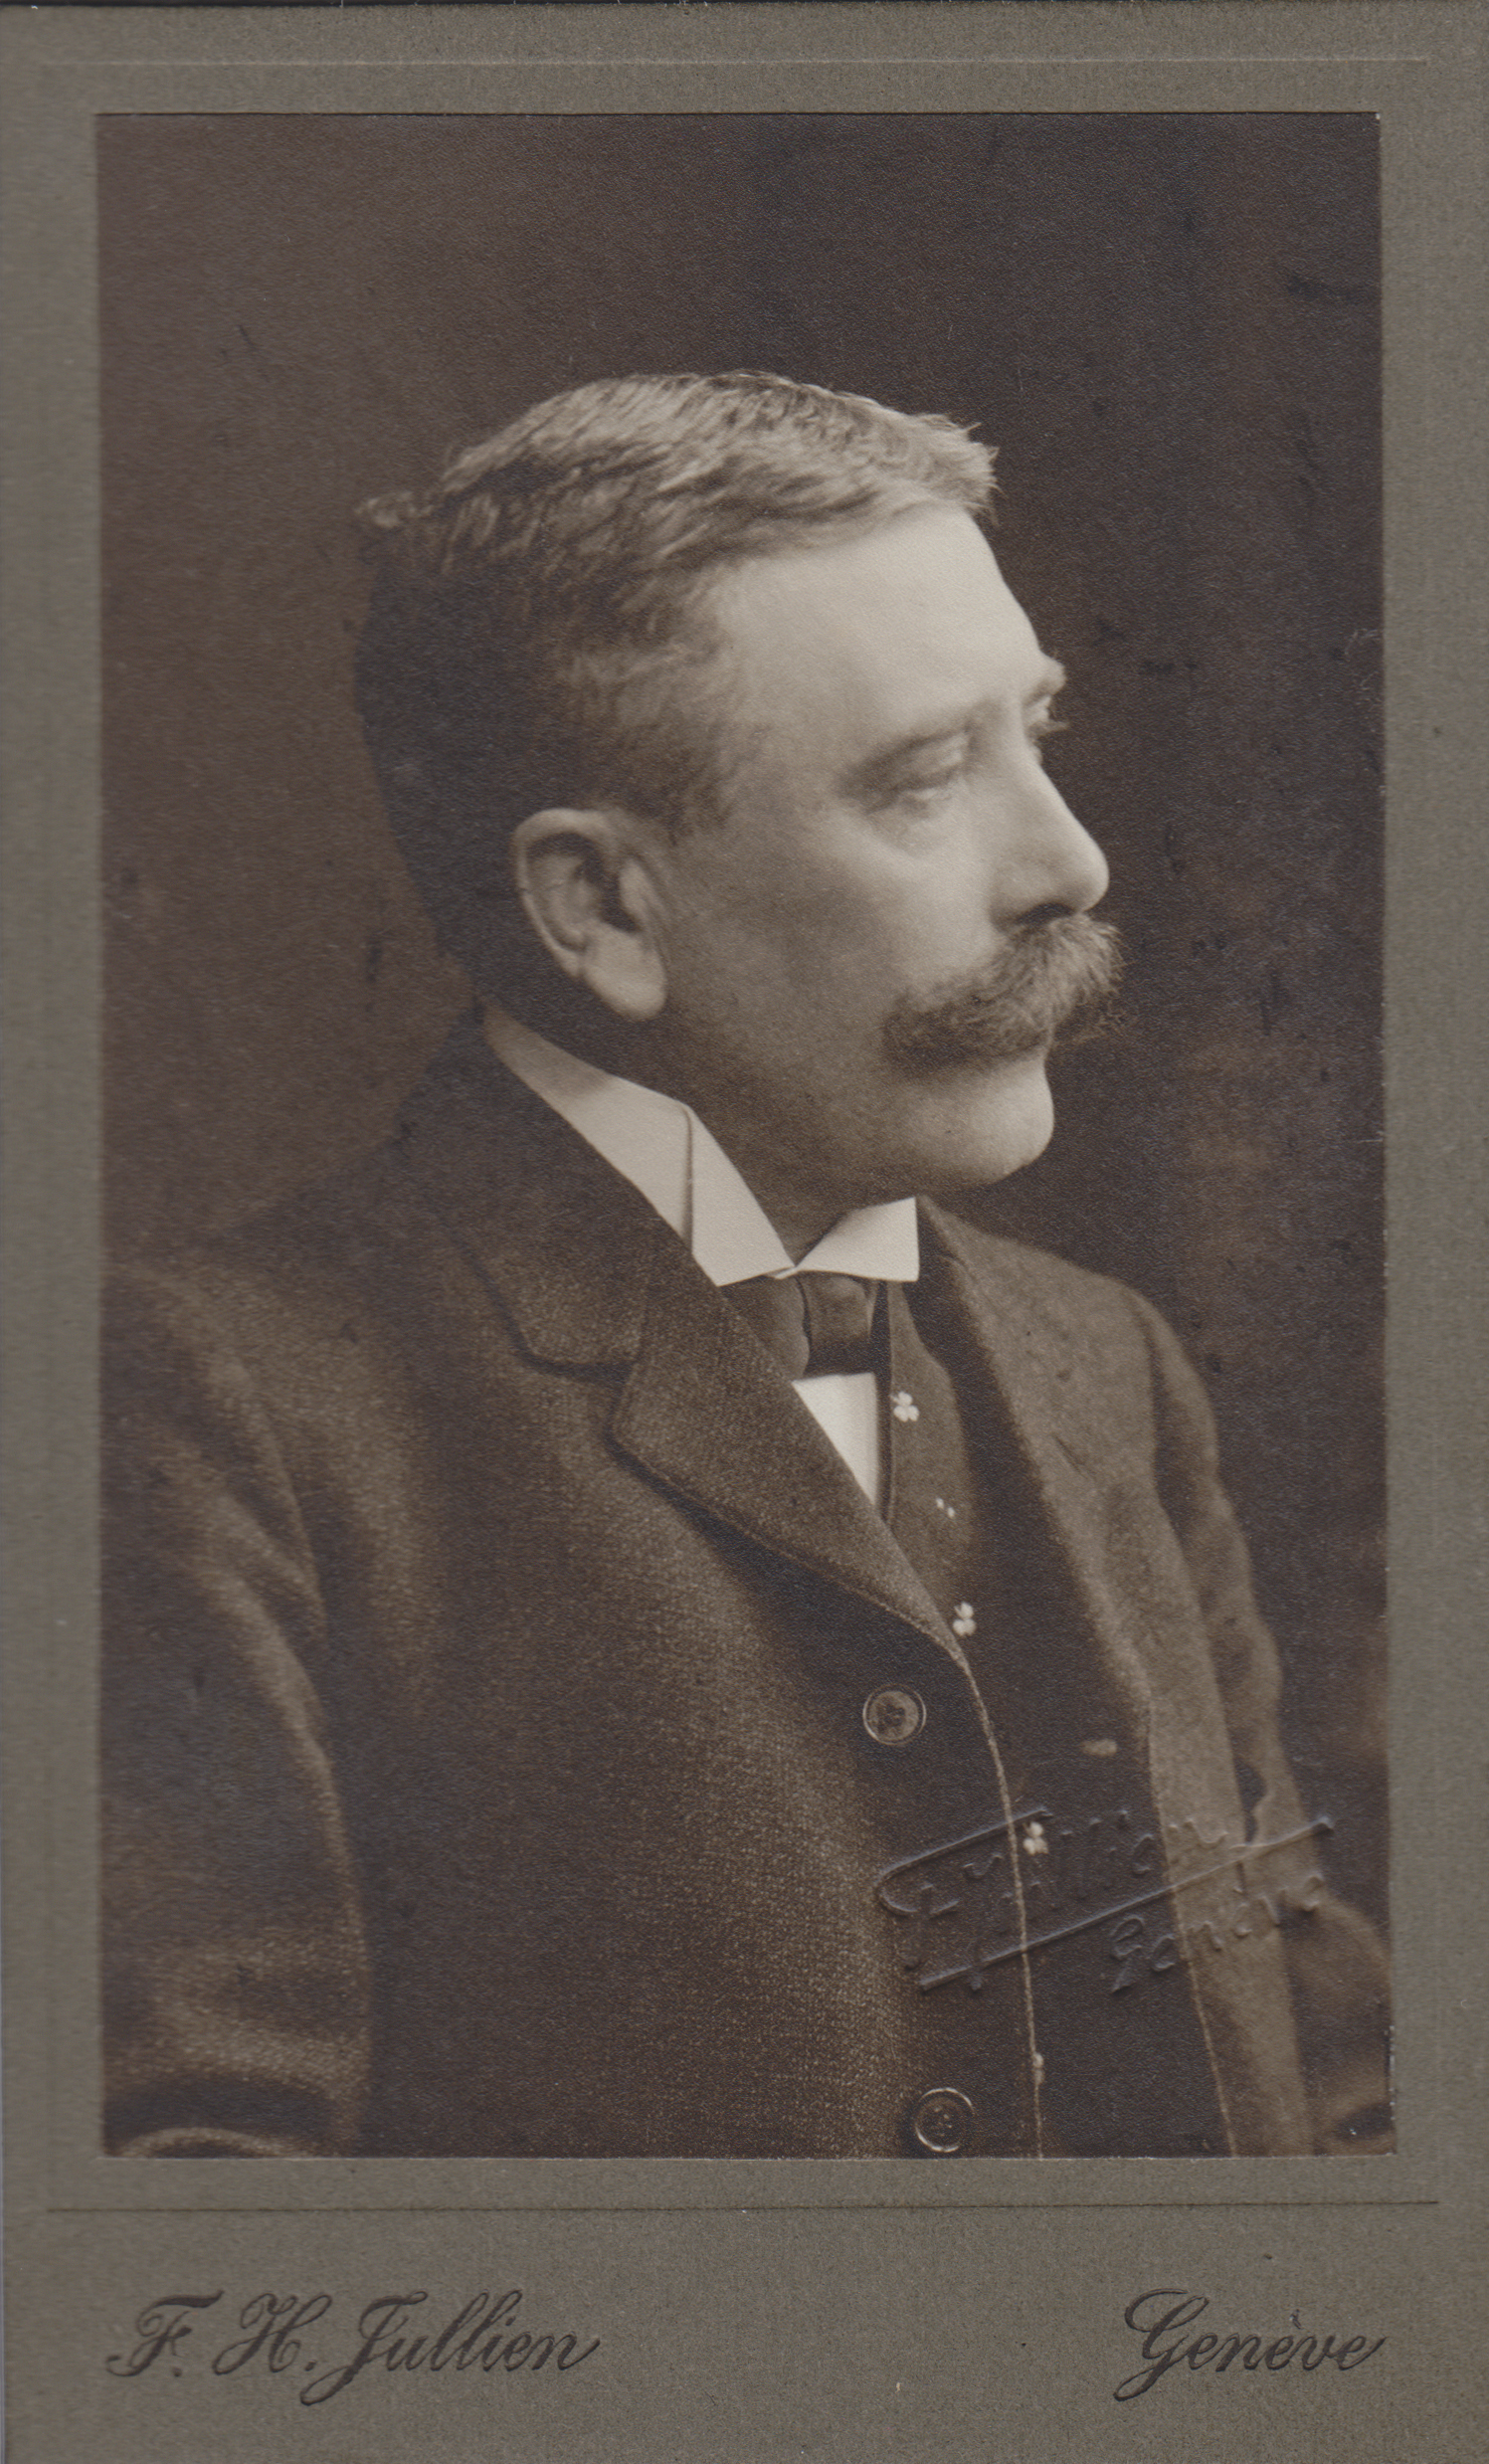
\includegraphics[width=.9\textwidth]{figures/DeSaussure.jpg}
  \caption{Ferdinand de Saussure}
  \label{fig:ch.saussure_sound.saussure}
\end{wrapfigure}
The reason for dwelling on these purely textual issues is that, while
{\Saussure}'s name conveys a sense of almost ultimate authority (at least
for some), finding out what his actual opinions were on concrete
issues is often all too much like the interpretation of the ancient
oracles. A very sparse and limited text drawn from presentation in a
context somewhat different from that in which it appears, full of
suggestion but lacking in specifics, and supplemented with isolated
unpublished notes, allows each interpreter to find what he wants, and
thus to legitimize his own picture of the problem. No doubt the
presentation in this chapter does not avoid such traps either, but
there seem to be some fairly clear points in {\Saussure}'s presentation
of phonetic problems, and I will attempt to stay as close as possible
to these.

\section{Sounds, sound images, and their study}
\largerpage
We can recall that {\Saussure} took linguistics to be the study of
systems composed of a certain class of signs, and that the signs in
question have the character of uniting a (\is{signified}) \isi{concept} with a
(\is{signifying}) \isi{sound image}. Most interpreters of {\Saussure} have attempted
to downplay the linguistic relevance of the sound images, but it seems
to me that to ignore the question of the specific character these have
is in a way to miss the point of {\Saussure}'s conception of language.

It is common, for instance, to cite the Saussurian doctrine that
``dans la \emph{\isi{langue}} il n'y a que des differences \ldots\ sans termes
positifs'' as evidence for the view that the particular elements
composing the sound system are not legitimately the object of
linguistic study. But to say that the linguist must be primarily
concerned with differences between sounds is not by any means to
reject entirely the study of the sounds themselves. While the
linguist's main interest is in the system of \isi{oppositions} between
signs, these \isi{oppositions} rest on the differences among sound images,
and these differences themselves reside in the character of the sounds
that are differentiated. {\Saussure} stresses that the study of the
formation and positive, physical character of sounds (the content of
traditional phonetics) is not in itself a linguistic study: it is only
when we consider the relations between sound images that we are
studying the system of language. But his insistence on the \isi{sound image}
as one of the two inseparable faces of the sign makes it clear that
insofar as their nature supports their differential function, these
sound images are indeed an aspect of the object studied in
linguistics.

We can perhaps make this issue more concrete by posing it in terms of
our usual conception of a grammar today. Within such a grammar, we can
identify two aspects of the description of the sound system of a
language. First, grammatical theory provides a set of phonetic
\isi{representations} for linguistic forms, in the form of a system of
\isi{transcription} together with the principles for its
interpretation. Such a system of \isi{transcription} is generally taken to
be fundamentally independent of any particular language, and its
definition is given in universally applicable terms based on human
linguistic capacities (rather than on the facts of an individual
language). Phonetic representation is often thought of as a sort of
neutral observation language for a class of physical phenomena, but
this is incorrect. In fact, systems of phonetic representation are
highly structured \emph{theories} of the phenomena of speech,
involving a number of systematic abstractions from the brute physical
facts \citep[68ff.]{sra:dwl:organ_book}.

Second, however, the grammar of an individual language provides a
system of {rules}, or principles particular to that language, which
characterize some of these \isi{representations} as (potentially) belonging
to different signs, and others as (potentially) belonging to the same
sign in Saussurean terms. `Redundancy {rules}', for example, in the
terminology of 1960s Generative Phonology, or similar constraint
mechanisms, specify that if the representation corresponding to a
given sign has some property P, it must also have (or, in some cases,
may not have) some other property P$\prime$. Such {rules} specify the
range of permissible \isi{variation} in the realizations of a given sign,
and thus (by implication) the characteristics that necessarily
differentiate distinct signs. There are, of course, other sorts of
regularity than those expressed in \isi{redundancy rules} or their
equivalent, and these are described by other mechanisms. The general
point should be clear: the {rules} of a language (as opposed to the
transcriptional system employed to represent phonetic forms) are
particular to that language, and, taken together, they characterize
the system by which sound differences correspond to \isi{oppositions}
between signs.

{\Saussure}'s point, formulated in these terms, is clear: it is the
business of the linguist to study not the nature of (phonetic)
\isi{representations} but the system of {rules} which underlies the
differentiation of signs and thus constitutes the sound system of a
particular language. Seen in this light, however, the sounds
themselves are anything but irrelevant to the task of the
linguist. Indeed, it is only on the basis of an understanding of the
nature of sound images that the task of formulating the {rules} making
up any particular system of signs can even be approached. We must
arrive at a proper conception of these sound images in order to have
an appropriate basis for the study of the system. For one thing, as we
will note below, they are identified less with an articulatory
characterization of utterances than with a somewhat more abstract and
`timeless' perceptual one. Yet they constitute the elementary units
whose differentiation is the basis of the \isi{linguistic system}.

It is sometimes suggested, nonetheless, that {\Saussure} felt signs to be
such abstract entities that the connection between the \emph{\isi{signifiant}} of a
sign and a \isi{sound image} per se is a completely accidental and
contingent fact, unconnected with the nature of language. Indeed, it
is insisted in the \textsl{Cours} that the material sound itself does
not belong to \emph{\isi{langue}} but is simply the substance which supports
linguistic expression (``phonation \ldots\ is only the execution of
the sound images''—cited by \citealt[82]{godel57:sources}), and thus is
a matter of \emph{\isi{parole}}. What is at issue here is the irrelevant or
accidental character not of sound images as is sometimes suggested,
but of sounds. These latter, for {\Saussure}, are particular physical,
articulatory implementations of linguistic possibilities, and thus
belong to the study of \emph{\isi{parole}}. Sound images, on the other hand, have a
timeless character as perceptual archetypes
\citep[98]{saussure16:cours-original}; and while these serve as the
basis of concrete acts of production or perception, they are not to be
identified with them. These sound images, as essential (though not
independent) components of the linguistic sign, are thus not excluded
from \emph{\isi{langue}}.

To this interpretation it might be objected that {\Saussure} explicitly
says that phonetic implementation of sounds is not necessary, since
the signs can be e\-voked by other means. It is, however, revealing to
note the example {\Saussure} uses to make this point: to wit, the
possibility of transposing linguistic signs into writing. On the face
of it, the expression of signs in writing has nothing whatsoever to do
with sound images, since it involves a completely different, visual
rather than auditory medium.

If we look at the context of this example in the notes on which the
\textsl{Cours} is based, however \citep[193f.]{godel57:sources}, the
issue appears in a somewhat different light. In fact, for {\Saussure},
writing bears a more or less direct relation (depending on the
particular system) to the system of sound images, taken in its
essential (rather than external, articulatory) character. The
\isi{segmentation} imposed by alphabetic writing systems, he feels,
corresponds to a fundamental property of sound images. This is a point
he makes explicitly in the \textsl{Cours} with regard to the \ili{Greek}
writing system: its \isi{segmentation} reflects the parallel \isi{segmentation} of
sounds in perception, which is imposed as a part of the essential
character of human \isi{speech perception}. Alphabetic writing thus provides
a sometimes imperfect, but largely accurate, representation of sound
images, just as the articulatory formation of concrete sounds
does. The relevance of the example of signs realized in writing, then,
is not that sound images are inessential to \emph{\isi{langue}} but that (physical)
sounds are. We must conclude, then, that an appreciation of {\Saussure}'s
views on the system of language must be founded, in part, on his
conception of the nature of sound images.

In the study of sound images, {\Saussure} distinguishes essentially three
ap\-proaches which can be seen as characterizing three distinct
fields. To a considerable extent, these divisions correspond to those
of later linguists, but although he often uses the same terms as those
appearing in later work, he uses them in radically different ways. For
the modern reader, the Saussurean terminology thus requires at least a
note of clarification.

The nature of the linguistic sign (especially its linear character)
and its realization in syntagmatic combinations leads directly to the
study of morphology, in approximately the sense of subsequent
linguistic theory. The spoken chain can be divided into discrete
signs, and morphology is the study of the principles underlying such
division. In various places, it is made clear that this organization
of the chain is based on (synchronic) proportional analogies, which
establish the relations between morphologically related words. As
noted in section~\ref{sec:linguistic-sign} of
chapter~\ref{ch.saussure_life}, and in clear i{contrast} with the views
of his brother René\ia{de Saussure, René} \citep{sra18:f.vs.r.saussure}, {\Saussure} is
reluctant to attribute independent existence to the subparts of words
isolated in this way, preferring to concentrate on the relations which
underlie the divisions. For our purposes here, it is sufficient to
note that divisions corresponding to different signs (some of which
are ``partially motivated'', or themselves internally complex) at
least the size of the word are assumed to exist and to be real to the
speakers of the language.

Individual signs in the spoken chain can be studied in terms of the
mechanisms and principles by which their sound images are realized in
speech, but this study is, by its nature, part of the linguistics of
\emph{\isi{parole}} rather than of \emph{\isi{langue}}. {\Saussure} calls this
\isi{synchronic study} of the \isi{articulation} and \isi{acoustics} of concrete sounds
\emph{phonologie}: it is essentially the same as what most linguists
would today call phonetics. In the discussion below, we will use the
modern terminology except where it is essential to call attention to
{\Saussure}'s usage (in which case we will refer to this discipline as
\emph{phonologie}).

{\Saussure} also distinguishes a discipline which he calls
\emph{phonétique}, but he uses that word in quite a different sense
than we do today. {\Saussure}'s \emph{phonétique} is not a synchronic
study at all; rather, it is the study of the historical evolution and
change of sounds. Like his \emph{phonologie}, it is an aspect of the
study of \emph{\isi{parole}}, since it is essentially based on the
mechanisms by which speakers realize the signs of their language in
concrete acts of speaking. {\Saussure} had considerable faith (as had the
\isi{neogrammarians}) that the detailed study of the facts of speech would
yield a comprehensive {explanation} of the mechanisms of sound
change. To conform more closely to modern usage, we will refer to this
study below as historical phonetics (except where {\Saussure}'s
terminology itself is in question).

{\Saussure}'s usage of \emph{phonologie} and \emph{phonétique} is
somewhat confusing to the modern reader, since essentially no one
other than his student \name{Maurice}{Grammont} (from his years in Paris) followed
his terminology. Nonetheless, both terms correspond to
well-established aspects of the study of speech. Neither one provides
us with a name for the study of sound images considered as a part of
\emph{\isi{langue}}, however. The sound images that form one aspect of the
linguistic sign differ from concrete sounds in essential ways (they
are timeless rather than being realized in time, they are neutral
between production and perception, etc.) and thus are not directly
accessible to either phonetic or historical phonetic study. In fact,
there is no reason to believe {\Saussure} had any word for the study of
the role of sounds in \emph{\isi{langue}}: this is simply an aspect of
linguistics. Indeed, since he emphasizes many times in his lectures
that the study of the linguistic sign must be based on the
\emph{simultaneous} study of the \emph{signifiant} and the
\emph{\isi{signifié}}, the pedagogical concerns which are so evident
everywhere in his presentation of fundamental problems would probably
have led him to avoid any term which would suggest an illicit
separation of one face of the sign from the other.

\section{`\textit{Phonèmes}' and `phonetic species'}

To understand the nature of sound images, let us {contrast} them with
the object of study in phonetics. Using the (not specifically
linguistic) methods of physical investigation, we can study the units
of sound in speech. These units have an articulatory side, and also an
auditory aspect (called `acoustic' by {\Saussure}): they thus have ``a
foot in each chain,'' as he puts it—which does not mean that they are
thereby neutral between the two ways in which we can study speech, but
rather that both sides are relevant to their character. These
concrete, actualized speech sounds, produced and perceived in real
time in acts of speaking, are called by {\Saussure} \emph{phonèmes}.

Of all of the divergences between {\Saussure}'s terminology and that of
later writers, this is undoubtedly the one which has given rise to the
most misunderstanding. While the word `\isi{phoneme}' in its incarnations in
various languages later came to designate a specifically distinctive
sound element, it is quite clear that {\Saussure} does not use it at all
in that way. Rather, he intends by the word \emph{phonème} simply a
`\isi{speech sound}', with no connotations of language-particular
distinctive character. When he speaks of the distinctive properties of
these elements, he means by this simply that it is in terms of
differences between speech sounds that the \isi{oppositions} between signs
are indicated in speech: this does not at all imply that the
\emph{phonème} itself is a unit whose content is limited to its
distinctive function, as later phonologists would come to use the
word.

In fact, for whatever historical interest this has, {\Saussure}'s use of
the word corresponds to its original sense. According to
\citet{mugdan11:phoneme,mugdan14:more-on-phoneme} (see also
\citealt{godel57:sources,Jakobson60:kazan.school}), the word was coined
(or at least introduced into the vocabulary of linguists) by the
Frenchman \name{Antoni}{Dufriche-Desgenettes}, along with a number of other
novel formations (which did not enjoy nearly as much success) in the
1860s, and was used without definition in presentations to the Société
linguistique de Paris in the early 1870s. 

Aside from a few papers delivered to the Société linguistique of which
either the text or a report appeared in its publications, we know
{\DufricheDesgenettes} primarily as one of the charter members of the
society. It is also recorded, however, that on one occasion he
proposed the repeal of the society's constitutional provision against
discussion of the origins of language (which he could not recall
having approved at the time); in the absence of a seconder, the
proposal was lost \citep[229]{koerner76:dufriche}.

In any event, {\DufricheDesgenettes} proposed the use of the word
\emph{phonéme} essentially as a substitute for the \ili{German}
\emph{\isi{Sprachlaut}}, and thus intended it simply as a designation of a
(unitary) sound. The word was taken up by other linguists in Paris
(e.g. \name{Louis}{Havet}), and {\Saussure} uses it in the \emph{Mémoire} (though
in yet another sense). In his work in general linguistics, it is clear
that it designates what we would today call phonetic segments,
considered as (ultimately unreducible) units in acts of speaking.

The integral and atomic character of {\Saussure}'s `\isi{phoneme}s' is
confirmed, for him, by the process of perception. On his view, when we
perceive speech it is directly in terms of a sequence of internally
homogeneous and atemporal acoustic impressions, corresponding to the
sequence of phonemes. In the face of the measurable continuity of the
speech signal, a process of \isi{segmentation} is thus seen as built into
the perceptual system (see the remarks above on the reflection of this
\isi{segmentation} in writing systems). Given the interest of
nineteenth-century phoneticians in the transitions and continuous
character of speech, this is a rather remarkable suggestion. {\Saussure}
cites no source for it, and takes it as a self-evident
observation. Nonetheless, it would be interesting to know where this
view came from.

Since the unitary percepts corresponding to phonemes are internally
homogeneous, we cannot analyze them directly. When we seek to describe
phonemes, therefore, we do so in terms of their articulatory face, by
describing the gestures of the vocal apparatus necessary to produce
them. The actual classification of phonemes on this basis which
{\Saussure} gives is based directly on the phonetic views of {\Jespersen},
with no particularly innovative features.

There is, however, a more abstract unit in phonetics than the
\isi{phoneme}. Pho\-nemes are, by their nature, articulated in combination in
the spoken chain. In particular, each \isi{phoneme} occupies a particular
place within a larger unit, the \isi{syllable}. By virtue of its position in
the \isi{syllable}, a \isi{phoneme} may have various characteristics which would
differentiate it from other, similar phonemes. The most extensively
described of these is the difference between \emph{implosive} (dynamically
closing) and \emph{explosive} (or dynamically opening) articulations. In
\ili{English} [dɪd], for example, the initial [d] is explosive, while the
final [d] is implosive: {\Saussure} would thus transcribe the sequence as
[˂dɪ˃d].

The articulations [˂d] and [˃d] are clearly distinct (quite
independent of any issues of \isi{voicing}, final release, etc.), and thus
explosive and implosive segments constitute different phonemes. The
differences between them, however, are based on the articulatory
organization of a higher level unit (the \isi{syllable}). When we abstract
away from the differences due to this factor, we arrive at the
phonetic species: a unit characterizable in terms of a
non-time-varying position of the articulators, and thus the sort of
description we usually give in phonetics. Both implosive [˃d] and
explosive [˂d] belong to the same phonetic species, [D]. There are
said to be a finite, though perhaps large, number of possible distinct
phonetic species, whose characterization is not dependent on a
particular language.

{\Saussure} appears to hold that the \isi{auditory impressions} corresponding
to pho\-nemes of the same phonetic species are the same, and thus that
this unit is closer to the auditorily basic unit in speech than the
\isi{phoneme} itself. Specific phonemes are the positional realizations of
phonetic species, where the variations among them are due primarily to
general phonetic, rather than language-particular,
principles. Fundamentally, it is syllabic organization that is being
idealized away from here, and one can easily detect the relation of
this view to the theory of \emph{coefficients sonantiques} presented in the
\textsl{Mémoire}. For example, one of the recurring examples of different
phonemes belonging to the same species is {\Saussure}'s description of
(prevocalic, onglide) [y], (vowel) [i], and (postvocalic off\-glide, or
second element of a diphthong) [i̯] as members of the same species
[I]. Aside from simple position in the \isi{syllable}, however, there are
other differences between phonemes that depend on their implementation
in combination with other specific neighboring phonemes, and that may
also be significant.

A comprehensive specification of the principles by which the same
phonetic species corresponds to different phonemes depending on its
specific position in the spoken chain would yield a sort of
`\isi{combinatorial phonetics}'. Ultimately, the possibility of explaining
historical changes within historical phonetics depends on the
development of such principles, since the occurrence of change in
\emph{\isi{parole}} is based on the detailed positional \isi{variation} between
phonemes. For example, {\Saussure} considers the sequences [..Vgn..] and
[..Vng..] (as well as other sequences of stop and sonorant) in the
history of \ili{Germanic}. The first (stop plus sonorant) developed an
epenthetic vowel, while the second (sonorant plus stop) did not (and
in this case, underwent \isi{assimilation}). If we ask why this difference
arose, we cannot provide an answer at the level of the phonetic
species, where the difference is completely arbitrary. In principle,
however, a consideration of the low-level \isi{variation} between the
phonemes involved would provide us with the basis of an \isi{explanation},
since the resonant preceding the stop would be formed differently (and
would thus be a different \isi{phoneme}) from that following it. A
corresponding difference would be present in the \isi{stops} as well, of
course.

Though {\Saussure} was not in a position to provide such explanations in
detail, he was clearly confident that a suitably worked-out theory of
\isi{combinatorial phonetics} would yield them. This faith that a
sufficiently minute study of (synchronic) phonetic detail would
furnish comprehensive explanations for phonetic change was a prevalent
attitude at the time, arising from a fusion of neogrammarian studies
on the regularity of \isi{sound change} with the increasing observational
sophistication of late nineteenth century phonetics. This notion of an
explanatory historical phonetics (as based on \isi{combinatory phonologie})
was carried considerably further in the work of one of {\Saussure}'s
Paris students \citep{grammont33:traite}.  It recurs (though perhaps
for completely independent reasons) in more current work, such as the
view of phoneticians like \name{John}{Ohala} (see, e.g.,
\citealt{ohala79:saussure}) that the substantive content of
\isi{phonological rules} can be exhaustively related to detailed facts of
phonetics. Apparently, however, this remains a research program rather
than a demonstrated proposition, just as it was in {\Saussure}'s time
(cf. \citealt{sra81:unnatural}).

\section{The linguistic representation of \textit{signifiants}}

Now that we have established the nature of the objects studied by
phonetics ({\Saussure}'s \emph{phonologie}), we can return to the
question of the nature of the \emph{\isi{signifiants}} of linguistic
signs. These are almost always referred to by {\Saussure} as \emph{images
  acoustiques}, or `sound images', and characterized as a psychic
reality that determines both the speaker's intentions and his
perceptions. The \isi{sound image} is thus neutral between production and
perception: it is the pattern which the speaker attempts to conform to
in production, and against which he matches external stimuli in
perception, but its nature is not to be identified with either the one
or the other. We can {contrast} this neutral character with the bivalent
nature of the \isi{phoneme}: the \isi{phoneme} is a concrete sound, and thus has
both a manner of production and a specific result in perception. The
\isi{sound image}, however, is neither produced nor perceived in individual,
concrete acts of speaking; rather, it determines the category to which
particular productions or perceptions are to be assigned.

When we speak, we attempt to produce a sequence of sounds that will
conform to the sound images of the signs we are employing. The
{mechanism} by which we do so is, strictly speaking, irrelevant to the
character of those sound images, and thus of the signs themselves. Our
listeners in turn perceive our speech as having a certain \isi{meaning}, by
virtue of the fact that the value-assigning properties of a sign in
their own system are activated when our acts of speaking conform to
its \isi{sound image}. The relation between sound images and particular
productions or perceptions is thus rather like that between
\emph{types} of elements and particular \emph{tokens} of those
types. Of course, having observed that the difference between sound
images and concrete sounds follows from their respective ontological
status, we have still not said anything very specific about what sort
of properties sound images have except that whatever these are, they
must be sufficient to support both production and perception when the
system of signs is employed in concrete acts of speaking.

In discussing the \emph{\isi{signifiants}} of linguistic signs, {\Saussure}
emphasizes repeatedly that what is essential to them is the fact that
they differ from one another. In the study of \emph{\isi{langue}}, our
interest is in characterizing these differences, which organize the
individual signs into a system of relations. This is really the
fundamental contribution which {\Saussure} made to the development of
linguistics: to focus the attention of the linguist on the system of
\isi{regularities} and relations which support the differences among signs,
rather than on the details of individual \isi{sound and meaning} in and of
themselves. This notion of \emph{\isi{langue}} as a system of relations is
entirely contrary to \posscitet[4]{chomsky:aspects} characterization of
{\Saussure}'s ``{concept} of \emph{\isi{langue}} as merely a systematic inventory
of items'', for example.

At the beginning of the twentieth century, this was a necessary and
timely shift in interest. The development of instrumental phonetic
techniques to replace earlier, largely introspective methods resulted
in studies so sophisticated that significance began to be lost in
phonetic detail. Once we recognize the range of aspects of a speech
event which it is possible to quantify, there is no apparent criterion
by which we can decide that a given amount of detail is enough. We
soon reach a point at which it is clear that while our measurements
may well represent true observations of the speech event, they no
longer represent things that are essential to its linguistic
function. Nothing in the physical event ({\Saussure}'s \isi{phoneme}) tells us
what is worth measuring and what is not.

{\Saussure}'s distinction between concrete sounds and the
\emph{\isi{signifiants}} of signs, however, throws such phonetic studies
into immediate focus: the linguistic function of a phonetic property
is determined by its role in separating (or not separating)
productions or perceptions corresponding to one sign from those
corresponding to another. For {\Saussure}, the detailed information
accumulated by phoneticians is of only limited utility for the
linguist, since he is primarily interested in the ways in which sound
images differ, and thus does not need to know everything the
phonetician can tell him.

By this move, then, linguists could be emancipated from their growing
obsession with phonetic detail. This still does not tell them much,
however, about what the sound images they are interested in are
like. The indication of (at least {\Saussure}'s conception of) their
nature, though, is to be found in their name: `\emph{images
  acoustiques}', by its content (and also by comparison with the
\emph{impressions acoustiques} associated with the perception of
concrete phonetic segments), suggests that these were simply idealized
\isi{phonetic representations}, fully specified for phonetic detail down to
the level of the phonetic species (though not to that of the
\isi{phoneme}). The difference between the \emph{\isi{signifiant}} of a sign, and
a phonetic representation (at the level of phonetic species) of an
utterance making use of that sign is thus a difference not in the
amount of information included but in the ontological status of the
characterization. As we suggested above, this difference is rather
like that between types and tokens.

The suggestion that the \emph{\isi{signifiants}} of signs are to be taken as
specified for a considerable range of phonetic properties is quite
contrary to the general interpretation in the literature of {\Saussure}'s
views. Because of his insistence on the central nature of the
differentiating properties of \emph{\isi{signifiants}}, it has been assumed
that these should be taken as specified only for their distinctive
properties. On this view, any property of a given phonetic species
which does not serve to distinguish one sign from another within a
given language should be left entirely unmentioned in the
representation of corresponding \emph{\isi{signifiants}} in that language
(though it would be specified, if distinctive, in the representation
of \textit{\isi{signifiants}} in some other language).

In fact, however, this notion of partially specified
\emph{\isi{signifiants}} is difficult to support on the basis of anything
{\Saussure} actually says. Nowhere does he say directly that a
representation of signs (or rather, of their \emph{\isi{signifiants}}) would
be fundamentally different in character (except for the difference in
ontological status stressed above) from a phonetic
representation. There is no suggestion, that is (even where he appears
to be raising the issue), that there is a need for a distinct
``phonemic'' representation in what would come to be the post-Saussurean
acceptance of this term.

Both what {\Saussure} says and what he does not say imply that
\isi{representations} of \emph{\isi{signifiants}} are fully specified (to the same
degree as phonetic species). For example, in discussing
transcriptions, he suggests that a fully detailed phonetic
\isi{transcription} (noting all of the properties of individual phonemes) is
really only useful for the physical scientist, and not for the
linguist. The reason presented for this, however, is not that such a
\isi{transcription} would include redundant detail, but rather that it is
clumsy and unaesthetic. A simpler representation, sufficient to
indicate phonetic species, is quite satisfactory for linguistic
purposes. We must remember that the representation whose linguistic
significance {\Saussure} is opposing is one whose degree of physical
precision is limited only by the ingenuity of the phonetician and the
accuracy of measuring instruments—not one which simply includes some
indication of properties which, while they may characterize a
particular phonetic species, do not happen to serve distinctively in
the individual language under investigation.

The interpretation of {\Saussure}'s ideas here may seem somewhat
paradoxical: after all, what characterizes a \emph{\isi{signifiant}} and
gives it its value within a given system of \emph{\isi{langue}} is what
distinguishes it from the other \emph{\isi{signifiants}} within that
system. Thus, the study of \emph{\isi{langue}} must elucidate the
distinctions or {oppositions} among signs, and it would appear that this
goal is not consistent with a representation of \emph{\isi{signifiants}}
which does not distinguish between distinctive and non-distinctive
properties in the \isi{sound image}.

This apparent difficulty results from confining our attention to the
role of \isi{representations} in a phonological description. To resolve it,
we must recall {\Saussure}'s general reluctance to attribute `reality' to
units that result from a linguistic analysis. Rather, he preferred to
assign `reality' to the relations which such an analysis reveals
between linguistic units. Returning to the conception of a linguistic
description as consisting not only of a set of \isi{representations} for
linguistic elements, but also a set of {rules} determining the form and
interconnections of these elements, we can see that the task of
elucidating the system of differences among signs might well be
construed as a problem to be solved by presenting the system of {rules},
without necessarily implicating the choice of a set of \isi{representations}.

\section{Some approaches to the study of phonological differences}

To make this suggestion somewhat more concrete, let us consider
several different ways in which one might undertake to describe the
differences among the (\emph{\isi{signifiants}} of) signs in a language. We
can characterize these theories in terms of the properties they assign
to a systematic notation for (language-particular) \emph{\isi{signifiants}},
which I will call a phonological representation, and the relation
between this notation and the rest of the description (the {rules}). As
will become clear in later chapters, all of the approaches to be
sketched below (as well as others, as we will see in
chapter~\ref{ch.structuralists}) have in fact been taken at various
times in the history of enquiry into \isi{sound structure}, and they are
thus not simply straw men.

At one extreme, we might decide to focus all of our attention on the
set of \isi{phonological representations} which the theory provides for
forms in the language. We would then, in essence, ignore the status of
{rules} in our description; but we could nonetheless come quite close to
a description identifying the properties which distinguish signs from
one another provided we could define \isi{phonological representations} so
that they will have exactly that character. On such a view,
\isi{phonological representations} would have to be specified only for the
distinctive properties of the forms they correspond to. While a
universally applicable theory of possible \isi{phonetic representations}
would presumably make provision for the indication of additional
properties, not distinctive in the language in question, those would
be `left blank' in the \isi{representations} of forms in this language.

On this view, for instance, all of the \emph{t}'s in \ili{English} words
like \emph{tip, step, pit, shirt}, etc. would simply be characterized
as voiceless coronal \isi{stops}, with no indication whether a given
\emph{t} was aspirated or not, released or not, apical or laminal,
etc. All that is indicated is the collection of properties that
distinguish \emph{t} from \emph{d, p, s} etc. Rules would then be
required to supply values for the other (non-distinctive) phonetic
properties of the segment under appropriate conditions.

Of course, we can imagine many implementations of such a theory,
differing in particular in the inventory of properties they recognize
as differentiating phonological elements (and particularly in the
relation between these properties and phonetically observable
ones). These differences are immaterial for the moment, since the
characteristic of such a theory to which we wish to draw attention is
its exclusive focus on defining `distinctiveness', `\isi{contrast}', etc. in
terms of the set of properties which are marked in phonological
\isi{representations} within a given language.

This sort of approach has characterized a great many versions of
`phonemic' theory in phonology. Such a theory describes the
differences between signs by defining a set of phonemes (no longer in
{\Saussure}'s sense), each of which is a segment characterized for all
and only those properties that set it apart from the other segments of
the system. A phonological representation then consists of a sequence
of such phonemes. Again, variations can be imagined: in some versions
of this theory, for example, additional properties may be extracted
and left unmarked when they are predictable within specific sequences
of phonemes (thus, otherwise-distinctive point of \isi{articulation}
features in a {nasal consonant} may be omitted when it precedes an
obstruent). For our purposes, what matters is that some criterion for
`distinctiveness' of a property, once given, is implemented as the
definition of a notation which is free of all nondistinctive
properties.

Of course, we must then define the relation between the phonological
notation and the phonetic reality it stands for. This relation is a
matter of a set of (in practice, often unstated) {rules}, which have the
function of `filling in the blanks' in the phonological
representation: i.e., adding nondistinctive properties to the set
which can be directly projected from the phonemic form. These {rules}
are in some ways similar to those evidently posited by {\Saussure} to
relate phonetic species to phonemes by adding phonetic detail which
arises as a result of the combinatory environment in which a given
segment is realized. {\Saussure}'s {rules}, however, are clearly not to be
construed as part of the system of any particular language. They are
rather a consequence of the (purely phonetic) universal {mechanism} of
human speech production. As an aspect of \emph{\isi{parole}}, they do not
belong to the system of \emph{\isi{langue}} in either the general or the
language-particular sense. The phonemic {rules} required by the theory
outlined above, however, are clearly not the same for all languages.

Phonemic \isi{representations} of the sort posited on the approach under
consideration \emph{are} a part of the system of \emph{\isi{langue}},
however, and if these must be completed by a language-particular set
of {rules} which specify them for additional (nondistinctive)
properties, the question still arises of which aspect of language such
{rules} should be regarded as belonging to. One extreme interpretation
would have it that only the \isi{phonemic representations} belong to
\emph{\isi{langue}}, and that the {rules} as well as the phonetic realizations
of forms belong to \emph{\isi{parole}}. In the long run, however, this is a
difficult view to maintain. Many scholars have pointed out that the
range of possible pronunciations of a given form is very much a part
of the language in which it occurs. Even if all of the distinctive
properties are produced correctly, a \isi{pronunciation} which makes
arbitrary changes in the nondistinctive properties must be excluded
\emph{by virtue of the system of the language in question}. This means
that the principles which determine such nondistinctive properties
must themselves be considered a part of the system, and thus of
\emph{langue}. It is very easy, however, to fall prey to the
temptation to disregard the existence (or at least the systematic
status) of these {rules} altogether, and to focus attention exclusively
on the definition of a language-particular non-redundant phonemic
representation for forms—as witness most of the phonemic theories of
the twentieth century, which have paid little or no attention to
anything except the appropriate definition of phonemes as elements of
\isi{representations}.

It is certainly such an interpretation which has most generally been
given to {\Saussure}'s views, on the basis of his emphasis on
distinctiveness coupled with his general lack of specific discussion
of how to go about describing it. For many interpreters, the only
conceivable way to realize {\Saussure}'s requirement that the system of
sign-differentiating distinctions be the object of linguistic
description was to define a representation with precisely that
character. We have suggested above, however, that this is not a
necessary interpretation of {\Saussure}: on the one hand because he seems
to speak of the \emph{\isi{signifiant}} of a sign in a way that implies a
less abstract, more `phonetic' description, not limited to distinctive
properties, and on the other hand because of his general reluctance to
set up a unit of analysis (here, the `\isi{phoneme}' in the post-Saussurean
sense) and attribute reality to it. Yet he certainly felt that
linguistic signs, and thereby their \emph{\isi{signifiants}} and
\emph{\isi{signifiés}}, are `real' if anything in language is.

A view of the sort just discussed can be called an incompletely
specified \isi{phonemic theory}, intending thereby that the phonemes are
specified only for a limited range of properties (not that the theory
is itself incompletely specified!). Its basic characteristic is that
the elements of a phonological representation (the `phonemes') are
rather abstract elements, in the literal sense that they abstract away
from some of the essential phonetic properties of actualized
speech. Such an approach is not, however, the only way to realize
{\Saussure}'s basic insight about the importance of the difference
between distinguishing and non-distin\-guish\-ing properties. We might
also imagine a theory centering on a somewhat more concrete notion of
what `phonemes' are. Such a position could be developed in
quasi-mathematical terms along the following lines:

Suppose that we have identified all of the phonetic segments which
appear in utterances in a given language. Call this the class
$P = \{p_{1}, p_{2}, \ldots\}$. Now suppose further that we have
identified whether, for each pair $(p_{i}, p_{j})$ in $P$, the
difference between $[p_{i}]$ and $[p_{j}]$ is capable of
distinguishing one sign from another in this language (i.e., in
presystematic terms, whether $[p_{i}]$ and $[p_{j}]$ \isi{contrast} or
not). Now let us divide the set $P$ into subsets, such that each
subset $P_{i}$ consists of at least one element $[p_{i}]$ from $P$,
together with all (and only) the other elements in $P$ that do not
\isi{contrast} with $[p_{i}]$. As a result (making some— possibly
strong—assumptions about the extent to which the relation of \isi{contrast}
is a well-behaved one), two segments $[p_{i}]$ and $[p_{j}]$ can be
said to differentiate signs (potentially) if and only if they belong
to distinct subsets $P_{i}$ and $P_{j}$.

Now from each one of the subsets $P_{i}$, let us choose exactly one
representative phonetic segment, designated as $[p_{i}^{*}]$. We can
call the set of $\{[p_{i}^{*}]\}$ the set of phonemes of the
language. For any utterance, its phonological representation is
derived by replacing each phonetic segment by its corresponding
\isi{phoneme}: i.e., by the `designated element' $[p_{i}^{*}]$ in the subset
$P_{i}$ of which the segment in question is a member. We can then give
a set of {rules} which would allow us to derive \isi{phonetic representations}
from phonological ones, by identifying the conditions under which each
of the members of a given noncontrasting subset $P_{i}$ occurs, and
replacing the designated member $[p_{i}^{*}]$ by other members of the
same $P_{i}$ under appropriate conditions.

Thus, on such a theory all of the \emph{t}'s in \ili{English} words like
\emph{tip, step, pit, shirt}, etc. would be represented by a single
designated member of the set of phonetic segments that do not \isi{contrast}
with \emph{t}: perhaps released, unaspirated apical {[t]}. Rules would
then replace this segment with other (phonetic) variants of \emph{t}
under appropriate conditions.

This view, which we will refer to as a \textit{fully specified basic
  variant} \isi{phonemic theory}, differs from an incompletely specified
\isi{phonemic theory} in at least two important ways. First of all, instead
of being identified for a small proper subset of the potentially
relevant properties of segments (namely, exactly the distinctive
ones), the `phonemes' on this view are fully specified phonetic
segments (though only a subset of those which appear in the
language). And, second, the {rules} of the phonology do not `fill in
blanks' in such an incompletely specified segment to arrive at a
phonetic form but, rather, replace one phonetic segment (the
designated one, or `\isi{phoneme}') with another.

It should be clear that this second view, while quite distinct from
the first, nonetheless allows us to satisfy {\Saussure}'s basic
requirement that the system of distinctions among \emph{\isi{signifiants}}
be described in the grammar. This is because, given any pair of
utterances, we can determine immediately whether or not they
correspond to distinct signs simply by comparing their phonological
\isi{representations}: if these are the same, the two could not be the
realizations of distinct \emph{\isi{signifiants}}, while if the phonological
\isi{representations} are different, they must be. This is essentially the
same as the way the notion of distinctness between \emph{\isi{signifiants}}
is reconstructed in an incompletely specified \isi{phonemic theory}: the
major difference between them is the fact that, if phonemes are taken
to be fully specified basic variants rather than incompletely
specified clusters of properties alone, it is much more obvious that
the {rules} (and not simply the \isi{phonemic representations}) of the grammar
play a significant role in the description of the \isi{linguistic system}.

Nonetheless, it is difficult to argue that such a conception of the
nature of phonological structure corresponds to that of {\Saussure}. We
have argued above that for him the representation of
\emph{\isi{signifiants}} ought to be in terms of sound images that
correspond to (specified) phonetic species, and in this respect the
\isi{fully specified basic variant} view corresponds better to {\Saussure}'s
apparent picture than does the incompletely specified variety of
\isi{phonemic theory}; but the notion of {rules} that replace one specified
segment type with another seems quite foreign to the presentation of
\isi{sound structure} in the \textsl{Cours} and other sources.

We might therefore propose a third variant of phonological theory,
which makes no distinction between a `phonological' representation and
the representation of forms as a sequence of (sound images of) fully
specified phonetic species. Such a theory would thus involve no
systematically abstract representation that pays special regard to the
notion of \isi{contrast}. Self-evidently, this is not enough: the single
representation assumed by this view does not suffice to solve the
fundamental problem of describing the system of differences among
\emph{\isi{signifiants}}. Given two such \isi{representations}, we have no direct
way of determining by inspection whether a difference between them
corresponds to a potential difference between signs, or whether it
falls within the range of permissible \isi{variation} in a single sign.

This function would thus have to be performed not by the `phonological
\isi{representations}' themselves but by a set of {rules} which specify both
the range of possible \isi{representations} in a given language and the
relations that obtain among such \isi{representations}. Such {rules} would be
similar (in part) to a set of \isi{redundancy} conditions applying to fully
specified forms, of the sort described in a generative framework by
\citet{stanley67:redundancy}. These include positive conditions
(`every form in this language has property P'), negative conditions
(`no form in this language has property P'), and implicational
conditions (`if a form in this language has property P, then it also
has property Q'). Among the latter, some conditions must admit
disjunctions, in order to allow for free \isi{variation} (e.g., in \ili{English}
`if a form ends in a stop consonant, this segment may be either
released or unreleased').

With this apparatus, we could claim to have fully captured the
difference between (potentially) distinct \emph{\isi{signifiants}} and
nondistinct variants. Given any two \isi{phonetic representations}, that is,
we are able in principle to determine their status in this regard by
an appeal to such a grammar. First, we ask whether either (or both)
violates any of the conditions stated as {rules} of the language. If so,
of course, such a form is not a potential \emph{\isi{signifiant}} at all,
let alone a contrastively distinct one. If not, we can then make an
inventory of the differences between the two forms.

Of course, if the forms do not differ at all (at the level of
`phonetic species'), we can claim that they could not correspond to
distinct \emph{\isi{signifiants}}. If they do differ, however, we can then
ask the following: is each individual difference between them related
to a permissible disjunction found within some rule of the grammar?
For instance, two forms in \ili{English} which differ only in that one has a
final unreleased stop where the other has a final released stop would
satisfy this criterion by virtue of the disjunction found in the rule
tentatively formulated above. If and only if there is some difference
between the forms which does not meet this condition, the forms
correspond to potentially distinct \emph{\isi{signifiants}}.

Though such a procedure may seem excessively complex when stated in
such detail, it should be clear that it is in principle just as
capable as the two preceding views of providing an explicit
reconstruction of the difference between distinguishing and
non-distin\-guish\-ing properties of \emph{\isi{signifiants}}. Its crucial
characteristic is the fact that it puts the whole burden of
elucidating this difference on the system of {rules} rather than on the
definition of a special sort of representation. On this view, the
business of the linguist is the formulation of such sets of {rules} for
particular languages—{rules} which represent the \emph{\isi{signifiants}} of
language-particular signs, and the relations between them, in a direct
fashion.

We do not mean to suggest that this third view of \isi{sound structure}
(which we can call a \emph{fully specified surface variant} theory) gives a
completely faithful picture of {\Saussure}'s own ideas. Nonetheless,
there are a number of respects in which it would seem to be at least
somewhat closer to those ideas than its competitors presented above.

By {contrast} with the `incompletely specified' phonemic view, it does
not require us to hypostatize the results of a linguistic analysis by
attributing reality to a `phonemic' representation distinct in
principle from the sound images that govern our linguistic use of
signs in production and perception. Everything that {\Saussure} says on
this issue implies that he did not conceive of the difference between
the form of the \emph{\isi{signifiant}} and that of phonetic reality as a
difference in degree of specification. Furthermore, as noted several
times above, he preferred as a matter of principle to treat relations
rather than abstracted units as having linguistic reality.

By {contrast} with the `\isi{fully specified basic variant}' view, however,
this last picture does not require us to posit {rules} that {change} one
segment type into another. As we will see below in the discussion of
his treatment of alternations, such a formulation of linguistic
\isi{regularities} would also be completely opposed to his basic notion of
synchronic linguistic structure.

A further potential advantage of the \isi{fully specified surface variant}
view of \isi{sound structure} is that it settles the question, posed above,
of what status non-distinctive properties have with respect to the
distinction between \emph{langue} and \emph{\isi{parole}}. If we formulate
the description of these nondistinctive properties as a matter of
language-particular {rules}, we are thereby attributing the range of
permissible \isi{variation} in phonetic species to the grammar of the
language, and thus to \emph{langue}. By {contrast}, the realization of a
sequence of phonetic species as a sequence of concrete phonemes (in
{\Saussure}'s sense) is a consequence of the human articulatory (and
perhaps perceptual) system, and thus a matter of \emph{\isi{parole}} to be
studied by phoneticians (although these details are also of interest
to the linguist insofar as they furnish the grounds for an explanatory
account of \isi{historical change}).

It would thus appear that there is a logically coherent alternative to
(post-Saussurean) phonemic theories as a way of realizing {\Saussure}'s
basic goals in the description of sound systems. More to the point,
there is also some reason to associate his views with such an
alternative, rather than with a theory based on the notion of the
\isi{phoneme} as a direct embodiment of linguistic \isi{contrast}. At minimum,
there is no reason to claim that {\Saussure} had a notion of the
`\isi{phoneme}' in the sense that term later came to bear, or that he would
have been better off if he had. Although on this view the
\emph{\isi{signifiants}} of signs, as phonetically specified entities, would
seem to have a positive character, this does not really separate such
a picture from any other (e.g., a strictly phonemic one) as long as
the elements of phonologically significant representation have any
properties at all (e.g., distinctive ones). In any event, it is not
the business of the linguist \emph{per se} to study the properties of
these \isi{representations}: that is a matter for phoneticians. The
linguist's interest is in the system of {rules}.

Indeed, one can maintain that the characterization of the system of
\emph{langue} on this account, since it consists simply in the
negative and oppositive specification of what limits there are on
\isi{variation} and what differences among forms are possible, comes as
close as possible to satisfying the Saussurean dictum that language is
form, not substance. By localizing the description of the system of
\emph{langue} in the system of {rules}, rather than in the
characterization of the entities which make up the \emph{\isi{signifiants}}
themselves, such a system based on fully specified surface variants
puts as much of the weight of \isi{linguistic description} as possible on
the description of linguistic forms and relations.

It is interesting in its own right to ask just how {\Saussure} conceived
of the sound-structural aspect of the system of linguistic signs. It
is also useful, because the very nonspecific nature of this side of
his theoretical presentation makes it possible to see his basic
insight in quite general terms which admit of a wide range of possible
realizations. Nonetheless, from the point of view of the history of
linguistics, such an inquiry is almost beside the point: what matters
about {\Saussure}, in a way, is not his own work (of which we have
precious little), but rather the infuence his perceived position had
on later linguists.

In fact, his interpreters paid almost exclusive attention to one
aspect of {\Saussure}'s thought: his insistence that a linguistic
description must be primarily a description of the system that
distinguishes one sign from another. Virtually all commentators
interpreted this project in the form of a notion of linguistic
representation (or `\isi{phonemic transcription}') which would reconstruct
distinctiveness directly. The result was the proliferation of
competing phonemic theories which we will see in later chapters,
nearly all claiming in one way or another to be directly inspired by
{\Saussure}'s basic insight. Arguably, all of these theories are
fundamentally misguided, at least from {\Saussure}'s own point of
view. There is no reason to believe that he construed the system of
\emph{langue} in terms of a system of representation: indeed, it does
not seem completely anachronistic to suggest that the fundamentally
relational character of \emph{langue} is closer in spirit to 
contemporary conceptions of a grammar as a system of {rules}.

\section{Saussure's description of alternations}

Another topic which is worth examining both for its own interest and
for its bearing on {\Saussure}'s general conception of linguistic
structure is his treatment of alternations. We have thus far focused
exclusively on the ways in which signs may be individually
differentiated, but of course {\Saussure} recognized that certain
recurrent differences between signs within a given language may have a
special status. When such differences are genuinely systematic, they
may serve not only to keep signs apart but also (somewhat
paradoxically) to link them to one another. The description of these
relations is intimately related both to his view of the structure of
\emph{langue} and to the nature of the connection between synchrony
and diachrony in language.

\begin{wrapfigure}[17]{l}{.4\textwidth}
  \includegraphics[width=.9\textwidth]{figures/Ferdinand_de_Saussure_by_Jullien_2.jpg}
  \caption{Ferdinand de Saussure}
  \label{fig:ch.saussure_sound.saussure_2}
\end{wrapfigure}
For example, in the history of \ili{Greek}, intervocalic [s] was lost as a
result of a \isi{phonetic change}. Roots originally ending in [s] thus came
to have two forms (with or without the [s]), depending on whether they
were followed by a vocalic ending or not. The systematic character of
the relation between forms such as \emph{tre-ō} and \emph{a-tres-tos}
led to the conception (for speakers of the language) that there was ``a
correspondence [..] between radical groups such as \emph{ne-/nes-},
\emph{geu-/geus-}, as representing equivalent groups''
\citep[47]{reichler-beguelin80:saussure-grec-et-latin}. Forms with and
without [s] could thus be related despite this difference in their
\emph{\isi{signifiants}}, and such a relation is called an
\isi{alternation}. Elsewhere, an \isi{alternation} is defined as a ``correspondence
by which two specifiable sounds permute more or less regularly between
two series of coexistent forms'' \citep[253]{godel57:sources}. The
reference to ``coexistent forms'' here is quite essential, since
{\Saussure} emphasizes at several places that an \isi{alternation} is a
grammatical phenomenon: ``an opposition of form to form, not of \isi{phoneme}
to \isi{phoneme}'' (\emph{Ibid}.).

Every view of phonology must come to terms in some way with the
phenomenon of \isi{alternation}, even if only by rejecting it entirely as a
principled aspect of \isi{sound structure}. The fashion in which \isi{alternation}
is viewed and formulated may be taken as one of the primary
`diagnostics' of a phonological theory. Much of the program of
generative phonology, for example, can be seen as founded on the
attempt to reduce alternating surface forms to unitary underlying
\isi{representations}. By {contrast} a number of different versions of
structuralist \isi{phonemic theory} can be distinguished from one another
largely in terms of the extent to which information about systematic
alternations is allowed to influence the choice of a phonemic
analysis.

The most obvious features of {\Saussure}'s attitude toward alternations
can be derived in large part from his (sometimes overstated) views on
the need to exorcise essentially diachronic facts from a synchronic
description. As an example of the consequences of this, consider a
common way of describing a pattern of \isi{alternation} such as that found
in \ili{Latin} \emph{capiō/percipiō}. It seems quite traditional to say that
\emph{percipiō} `comes from' \emph{capiō} by a rule that reduces [a]
to [i] in medial syllables. For {\Saussure}, however, this is completely
wrong, since it imports a number of confusions into the synchronic
system. Not the least of these is the impression that a historical
change (the \isi{sound change} by which [a] was replaced by [i] in medial
syllables) is somehow a part of the synchronic grammar.

On {\Saussure}'s view, the synchronic fact is simply a systematic
resemblance between two distinct signs (\emph{capiō} and
\emph{percipiō}). Both signs are part of the system of \emph{langue}
(as is the resemblance between them), but this does not mean that
either `comes from' the other. If \emph{percipiō} `comes from'
anything, it is earlier \emph{percapiō}, and this is strictly a
historical fact. The relation between earlier per \emph{capiō} and
later \emph{percipiō}, though, is not a fact of \emph{langue} but
rather a fact of \isi{phonetic change}, and thus a matter of
\emph{\isi{parole}}. 
As far
as the system of \emph{langue} is concerned, what has happened is
simply that the earlier opposition between the forms \emph{capiō}
vs. \emph{percapiō} has been replaced by a different one: \emph{capiō}
vs. \emph{percipiō}. At both stages, we have two distinct signs; and
though the character of the distinction changes from one stage to the
other, this change is not itself a property of the synchronic grammar
(of either period).

Sometimes the \isi{alternation} which results from a series of historical
changes may itself become an essential part of the \emph{\isi{signifiant}}
of a grammatical category. Thus, in early \ili{Germanic}, the opposition
between singular and plural in pairs such as \emph{fōt}
vs. \emph{fōti} was carried by a distinct, separable ending
\emph{-i}. As a consequence of the sound changes of \isi{umlaut},
unrounding, and final vowel loss, this was replaced in \ili{Old English} by
the opposition between \emph{fōt} and \emph{fēt}. At this point,
however, it would not be correct to say that \ili{Old English} \emph{fēt}
`comes from' \emph{fōt} by a synchronic rule of \isi{umlaut}: rather, the
language recognized the systematic character of the \isi{alternation} as a
possible relation between signs. Some signs whose \emph{\isi{signifiants}}
contain back vowels are systematically related to other signs
differing exactly in that their \emph{\isi{signifiants}} contain
corresponding front vowels. In pairs like \emph{fōt/fēt}, this
relationship is itself seized on as a basis for the signified
difference between singular and plural—just as any other difference in
\emph{\isi{signifiants}}, such as a difference in their initial segments, or
the difference between forms with and without a final [-əz],
etc. might have been the basis for this opposition. The relation
between forms, then, is a part of the synchronic system just as the
range of possible elements of sound images is.

Despite the fact that such a systematic resemblance is a part of the
synchronic grammar of the language, we must avoid saying that in pairs
like \emph{fōt/fēt} or \emph{capiō/percipiō} we have a single unit
(\emph{fōt}, \emph{capiō}) and a synchronic rule which changes this
into something else under specifiable circumstances. In fact, neither
at the later stage, where a systematic \isi{alternation} is present, nor
even at the earlier stage (where we had \emph{fōt} versus \emph{fōti},
or \emph{capiō} vs. \emph{percapiō}) did we have to do with a single
unit. In synchronic terms, we have at each stage two distinct signs
rather than a single unit. The `change' is a fact of historical
phonetics, ``but its action belongs to the past, and for the speakers,
there is only a synchronic opposition''
\citep[219]{saussure16:cours-original}. To state a rule that changed
one form into another would falsely give the impression of ``movement
where there is only a state.'' (\emph{Ibid}.)

Furthermore, it would be incorrect (according to {\Saussure}) to say even
that in the past there was a single unit in such cases, and that it
underwent two divergent phonetic developments. It requires some
reflection to understand this assertion, since it appears to be just
such divergent development of an original unity that he previously
invoked as the diachronic fact leading to the synchronic
\isi{alternation}. But in fact, he suggests, there was in every such case
some difference in the forms involved even at the earlier period, and
it is this difference which is accentuated (and not created) by the
\isi{historical change}.

This becomes clearer when we recall the importance {\Saussure} attributed
to the detailed study of combinatory phonetics, which would ideally
reveal the minute differences between similar phonemes appearing in
different positions in the \isi{syllable} or other suprasegmental unit. Even
if we had the same sequence of phonetic species in \emph{fōt} and
\emph{fōt(-i)}, that is, the non-identity of the two signs would lead
to differences among the detailed phonetic properties of the
corresponding phonemes. A [T] in final position is realized
differently from a [T] preceding [i]—and thus, the [ō] in \emph{fōt}
is in a different environment from that in \emph{fōti}, which could
lead in turn to a difference between these two [ō]'s. If we had rules
in our synchronic description which change one segment or form into
another, not only would we risk importing diachronic facts illicitly
into \isi{synchrony}, but we might also be led to overlook a potential
phonetic {explanation} of the change. For {\Saussure} that {explanation}
proceeds from the original difference between forms and not their
unity.

{\Saussure}'s categorical rejection of the description of alternations by
a unitary `underlying' form and rules changing one segment into
another had very important consequences for the development of the
field. Subsequent generations of linguists, feeling that this
rejection followed directly from the cogency of the distinction
between synchronic and diachronic linguistics, adopted it as well. As
a result, it was quite some time before any sort of `morphophonemic'
account was considered a respectable part of a \isi{linguistic description}
again. {\Saussure} limited the characterization of \isi{alternations} to a
description of differences among surface forms, and in this he was
broadly followed (with some few exceptions which we will note in
following chapters). As a result, the general topic of alternations was
taken to be the matter of higher level studies (i.e., morphology)
rather than a question of \isi{sound structure}. The limitation on a
particular technique of description which {\Saussure} argued for was thus
interpreted as a limitation on the range of data relevant to a
phonological analysis: a much stronger restriction.

We must emphasize that, while {\Saussure} had no sympathy for a
description of alternations which posited unitary underlying forms and
rules altering the character of segments, he certainly considered
alternations to be a rule-governed aspect of \isi{sound structure}. Rather,
he took the rules involved to be ones which directly related one
surface form (in a given language) to another, without assigning
priority to either (or setting up an indirectly attested third form
from which both are derived). As such, all of his rules have the
character of `\isi{lexical redundancy rules}' (in the sense of
\citealt{jackendoff:wfrs}) or `correspondences' (in the sense of
\citealt{lopez:thesis}). A rule of this character may state an
inferential relation between forms (`if the language contains a form
with the properties \{$F$\}, then there may also exist a
systematically related form with the properties \{$F\prime$\}'), but
the relation is stated directly between the forms involved rather than
in terms of derivations of either or both from some other (possibly
more abstract) \isi{representations}.

Such a nonderivational characterization may or may not be an
appropriate way to describe alternations in the general case, but that
is not the issue here. What is important to note is that {\Saussure}
attributed considerable importance to the description of alternations,
and he was certainly ready to attribute `reality' to the rules which
described them. This reality was confirmed, in his view, by the
phenomenon of \isi{analogy}.

It will be recalled from section~\ref{sec:diachrony} of
chapter~\ref{ch.saussure_life} that for {\Saussure} the category of
`\isi{analogical change}' did not constitute change in the system of
\emph{\isi{langue}} at all, since he viewed analogical formations as
consisting simply in the realization of latent possibilities inherent
in the system of \emph{\isi{langue}} as it already exists. When a child uses
the form \emph{goed} instead of \emph{went}, this does not constitute
a change in the system, since the system already contains a rule to
the effect that, corresponding to a given present tense verb base,
there may be a past tense form which is the same with the addition of
the suffix \emph{-ed}. The form is thus inherent in the system, and
the child's use of it does not constitute change. Of course, if the
form \emph{goed} eventually comes to replace the form \emph{went}
entirely, the loss of this latter sign does constitute a change, but
the creation of the analogical innovation does not.

In order for this account of \isi{analogy} to go through, it is necessary to
recognize a wide range of alternations as encoded in the principles of
the system of \emph{\isi{langue}}. Furthermore, at least in principle, it
imposes a significant constraint on the operation of \isi{analogy}, since an
analogical formation is only possible insofar as the language contains
(independently) a rule of \isi{alternation} which supports the creation of
the innovated form. Not simply any four-term proportional such as
$A : A\prime\ = B : X$ is potentially a valid \isi{analogy}; the proportion
can only lead to the creation of an analogical form if a) some rule of
the grammar relates $A$ and $A\prime$, and b) the same rule
(potentially) relates $B$ to some other form $B\prime$ ($=X$). This
limitation would prohibit, for instance, the creation of a new verb
\emph{heye} `see' in \ili{English} on the basis of the proportion \emph{ear}
: \emph{hear} = \emph{eye} : $X$. Such a spurious proportion could not
be the basis of a possible analogical creation for {\Saussure}, since the
relation between \emph{ear} and \emph{hear} is quite isolated in
\ili{English}, and not based on any rule of the grammar. {\Saussure}'s position
on the fundamental relation between possible analogies and existing
rules of grammar is quite close to one that would be developed more
explicitly by \citet{kurylowicz:laws,kurylowicz:ieinflection}.

The interplay of the system of rules in determining the operation of
\isi{analogy} is carried quite far in some of {\Saussure}'s concrete
discussions. A standard example of analogical creation is the
replacement of \ili{Latin} \emph{honos} by \emph{honor}, on the basis of the
proportion ``\emph{ōrātōrem : ōrātor = honōrem : x}''
\citep[226]{saussure16:cours-original}. The discussion of this example
in his \ili{Greek} and \ili{Latin} phonology course, however
\citep{reichler-beguelin80:saussure-grec-et-latin}), shows that more
is involved here than simply the existence of the three terms of which
the proportion is composed.

In particular, the \isi{historical change} of ``\isi{rhotacism}'' in \ili{Latin} had
changed intervocalic instances of [s] into [r] (the detailed history
of this change need not concern us here). As a result, many forms
(such as \emph{honōs/honōrem}) showed an \isi{alternation} between [s] and [r]
under determinate conditions, and this was, for {\Saussure}, reflected as
a rule of the grammar of \ili{Latin}. However, many other forms (those with
original [r], not [s]) showed an [r] that did not alternate with
[s]. In these forms, intervocalic [r] was regularly related to final
and preconsonantal [r].

Now given a form with intervocalic [r] (such as \emph{ōrātōrem} or
\emph{honōrem}), one could not determine directly from it whether the
[r] in question was one that alternated with [s] or not. {\Saussure}
suggests that it is precisely this indeterminacy (which we would today
label `\isi{opacity}', after the proposals of
\citealt{kiparsky:3dimensions}) which provides the motivation for the
analogical formation. This consists in substituting the \isi{regular}
pattern [r] : [r] for the \isi{alternation} [r] : [s]. Both patterns are
justified by rules of the grammar (one trivially, and the other by the
synchronic, relational residue of \isi{rhotacism}). The choice of the
pattern [r] : [r], and thus the `creation' of \emph{honor}, is
explicitly said to be due to the fact that ``un paradigme tend a
unifier le cadre dans lequel il court''
\citep[56]{reichler-beguelin80:saussure-grec-et-latin}. An appeal to
the tendency of paradigms to be simplified is thoroughly traditional,
of course, but {\Saussure}'s use of it here to predict the way in which
an opaque interaction of rules will be resolved is rather similar to
that found in more recent discussion.

Though {\Saussure} does not explicitly point out the limitation of
analogies to those based on existing synchronic rules, it follows from
his conception of analogical `change', and it is reasonably clear that
he adhered to it in those places in which the problem arose (such as
his lectures on \ili{Greek} and \ili{Latin} phonology and morphology). His
formulation of particular analogical developments frequently involves
an appeal to the rule-governed character of the \isi{alternation} which
supports them; and his rejection of other proposed accounts in terms
of \isi{analogy} sometimes rests on their lack of such a foundation. It is,
obviously, difficult to delineate \emph{a priori} just when a resemblance
between forms justifies positing a rule of the grammar. It is
therefore difficult to be sure that all of {\Saussure}'s specific
historical discussions are in accord with his principle. This
difficulty is by no means unique to {\Saussure}'s view, however. What is
essential to recognize about his picture is that in principle, \isi{analogy}
is directly linked to the structure of the grammar, and in particular
to the pattern of systematic alternations that form part of a given
system of \emph{\isi{langue}}.

\section{Saussure and the phonological tradition}

This concludes our review of the principles of {\Saussure}'s phonological
views. While there is very little in his work which is specific enough
to serve directly as the foundation for concrete descriptions of
phonological structure, most of the issues that have occupied the
field since are at least raised, and a number of them have their
origins there. We hope to have shown above that {\Saussure}'s conception
of the system of \emph{\isi{signifiants}}, which makes up la \emph{\isi{langue}},
not only was not simply an inventory of signs, but also was not
primarily in terms of a special sort of notation or representation for
forms, but rather in terms of a system of rules which define the
interrelations among forms. These include rules delimiting the range
of forms in a particular language together with the range of \isi{variation}
permitted within the realizations of the same \emph{\isi{signifiant}}, and
also describing the patterns of systematic \isi{alternation} that relate one
form to another within the system. All of these are aspects of the
system which {\Saussure} felt was real for individual speakers, and which
formed the basis of the social, interpersonal character of language.

We do not intend to give the (anachronistic) impression that
{\Saussure}'s views were `wholly modern', of course. Among other clear
limitations which set his system apart from much of today's work in
phonology, his `rules' were limited to the statement of unmediated
\isi{regularities} obtaining within and among surface forms, rather than
deriving these (in at least some cases) from more abstract forms.

Other differences as well separate {\Saussure} from phonologists of
today. However, there is also a great deal he has in common with later
phonologists, as well as a great deal that separates him from those
who would come immediately after him (frequently invoking his name as
the basis of their work). Aside from the introduction of principles
(which often became mere slogans) such as the distinction between
\emph{\isi{langue}} and \emph{\isi{parole}}, the separation of synchrony from
diachrony, and the \isi{arbitrariness} of the linguistic sign, {\Saussure}'s
influence was primarily felt in a major redirection of efforts in
linguistics. Where these had previously been aimed at somewhat
atomistic historical studies based on phonetic detail, subsequent work
has concentrated on the study of systems, of synchronic \isi{regularities},
and especially of what is characteristic (perhaps universally) of
overall language-particular grammars.

In all of these respects, later studies came to be founded on
{\Saussure}'s own principles (though the same cannot be said, it would
seem, for the attempt to realize these goals largely through the means
of defining a theoretically significant level of representation). As
we noted in the introduction to chapter~\ref{ch.saussure_life},
however, {\Saussure} himself probably served more as the incarnation of a
program which was in some sense `in the air', reinforcing and
legitimizing these views in others rather than constituting their
substantive source. While the extent of his direct influence remains
to be established with certainty, it appears to have been exerted in
large part \textit{ex post facto}.

%%% Local Variables: 
%%% mode: latex
%%% TeX-master: "/Users/sra/Dropbox/Docs/Books/P20C_2/LSP/main.tex"
%%% End: 
